\section{Terrain Generation Using Procedural Models Based on Hydrology}
\label{sec:Hydrology}
Previously we introduced an approach that made use of local terrain features in various combinations to create terrains. This process was not procedural and heavily depended on the artists creativity to place and scale local features. In \cite{Genevaux:2013:TGU:2461912.2461996} a more modest approach is introduced, which generates a terrain procedurally around a given set of features, namely river networks.
 
\subsection{River Network Generation}
A river network can be interpreted as a graph, whose nodes act as either a spring, river mouth, or as a fork. 
The first step is to create a set of initial candidate nodes on the contour $\Gamma$, which act as river mouths. The user can additionally sketch some parts of the rivers. Initial nodes are placed on regularly jittered sample locations on the sketch. Each node is assigned a priority index, defining the overall appearance of the resulting river network hierarchy. 

\begin{figure}[htb]
	\centering
	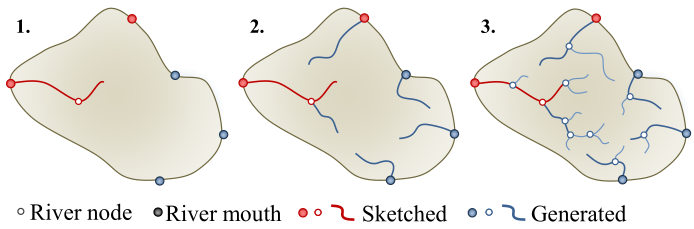
\includegraphics[width=\linewidth]{GGG13/river_network_sketch}
	\caption{Successive growing of the river graph. }
	\label{fig:river_network_sketch}
\end{figure}

For generating the network, the geometric graph $G$ is incrementally grown and elevated using a probabilistic approach. For each candidate node in $G$ the following steps are performed. 
\begin{enumerate}
	\item A \textit{Node selection}: choose a node $N$ from $G$ to which will be expanded.
	\item \textit{Node expansion}: expand the choosen node and perform geometric tests to verify its compatibility with the previouly created nodes. 
	\item The \textit{Node creation}: add the expanded node $N$ to $G$ 
\end{enumerate}

\subsubsection{Node selection}
The node that will be expanded, is selected using a heuristic that takes the elevation and its priority index into account. The combination of the two criteria allows a simultaneous creation of multiple networks competing for space. 
First we find the candidate node with the lowest elevation $z$. 
$\zeta $ is a parameter, that controls maximum range of elevation. Therefore we obtain a subset of admissible nodes, that are within the range of $[z, z + \zeta]$. From this set, the node with the highest priority index is chosen. If more than one node satisfies this criterion, the node with the lowest altitude will be chosen. 

Therefore the value of $\zeta$ directly influenced the appearance of the networks. If the decision is mainly based on the priority index (large $\zeta$), large networks are created. In contrast, if the elevation is pivotal, many local networks of similar sizes are created.

\begin{figure}[htb]
	\centering
	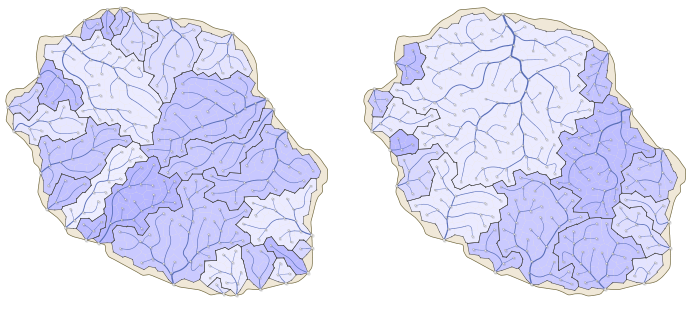
\includegraphics[width=\linewidth]{GGG13/drainage_system}
	\caption{Different networks are obtained from different $\zeta$ values. With $\zeta = 0$, we obtain networks of similar sizes. When using a high value $(\zeta = 20)$, one large network suppresses other networks. }
	\label{fig:dif_networks}
\end{figure}

\subsubsection{Node expansion}
To guarantee a consistent water flow, the elevation of a new node hast to be higher than its ancestors. This can either be achieved by using a river slope map. Such a map describes an intuitive way of how the network will expand. The probabilities $P_a, P_s, P_c$ for asymmetric branching, symmetric branching, or simple continuation without branching have to be predefined. 

To determine whether an expansion is valid, the system uses Horton-Strahler numbering. The Horton-Strahler number of a leaf  is $s$ = 1. An inner node inherits the maximum Horton-Strahler number from its children. If more than one children share this number, the Horton-Strahler number gets increased by 1.

For evaluation the tree is populated with the priority indices of the nodes. Using the probabilities  $P_a, P_s, P_c$ the type of the selected node is compared its possible new neighbour. Additionally the geometric properties of the graph are checked in order to prevent invalid nodes causing collisions and loops.  
\begin{figure}[htb]
	\centering
	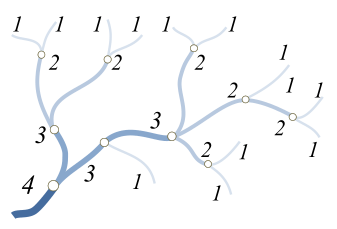
\includegraphics[width=0.5\linewidth]{GGG13/horton-strahler}
	\caption{Horton-Strahler numbering.}
	\label{fig:horton_strahler}
\end{figure}

\subsection{River Classification}
Once the river graph is build, the domain is divided into non overlapping cells, computed from the Voronoi diagram of node locations.  
The watershed of a cell $s$ is defined as the set of upstream connected cells and are associated with each water outlet of a cell. Its area is approximated by the sum of areas of cells connected to s. This is used to calculate the mean flow of the river. 

\begin{figure}[htb]
	\centering
	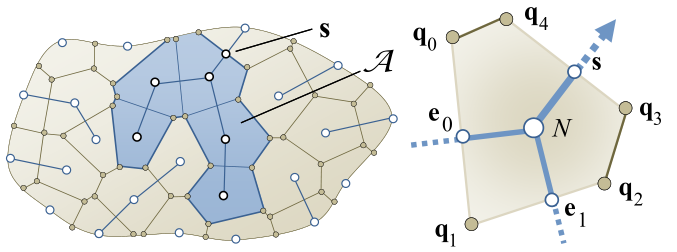
\includegraphics[width=\linewidth]{GGG13/voronoi_watershed}
	\caption{Example of watershed(blue) and a Voronoi cell.}
	\label{fig:voronoi_watershed}
\end{figure}

An edge of a Voronoi cell intersecting the river graph carry a connection to other river cells. Therefore the edge cannot be elevated. Edges that do not intersect the graph are used to compute the elevation of ridges between several streams. The points of this edge are called crest points. Each crest points is located at an equal distance $d$ from the centers $a, b, c$ of neighboring river nodes. Looking at figure \ref{fig:crest} the crest q should have a higher elevation than $a$, $b$ and $c$, insuring a continuous water flow. The elevation $q_z$ is computed as follows: 

$$q_z = max(a_z, b_z, c_z) + \lambda(q) \cdot d, \\ \lambda \in [0; 0.25]$$ 

$\lambda$ describes a slope magnitude function that describes if the terrain is mountainous. This terrain slope map can be set by the user or generated prodedurally. 
\begin{figure}[htb]
	\centering
	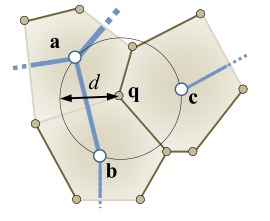
\includegraphics[width=\linewidth]{GGG13/crest}
	\caption{Calculation of the crest elevation.}
	\label{fig:crest}
\end{figure}

Each cell is assigned a class label, that corresponds to the type of river. Each class has a trajectory type and a digging profile of the riverbed. It includes geological composition of the riverbed. Each node is assigned such a label based on the river slope, and its proximity to the coast. 

\subsection{River Primitives Generation}
Each cell gets represented by a primitive. First all junctions are generated in a cell. The process starts by connecting two neighbouring water entries inside the cell. Incrementally all consecutive entries are added to the previous stream. Finally the stream is then connected to the water exist. The connection angle of two rivers is defined by the amount of water flow in the streams. Junctions of two rivers with the same size will cause a small junction angle, whereas a vastly difference in water flow will result in an almost perpendicular angle. 

\subsection{Terrain Model Generation}
Each river class has predefined profiles and a base trajectory of river flow. Using this information, the terrain primitives are generated with the same approach presented in section ~\ref{sec:tmffp}. This allows for additional terrain features and noise textures to be combined with the river flow, to create realistic looking terrains. 
\begin{figure}[htb]
	\centering
	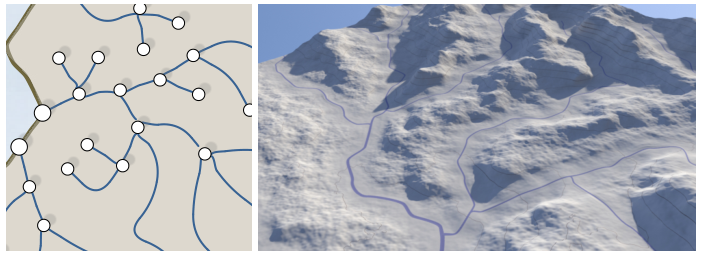
\includegraphics[width=\linewidth]{GGG13/valleys_and_rivers}
	\caption{Rivers and valleys created with a river graph.}
	\label{fig:valleys}
\end{figure}
